	\chapter{Structure mécanique}
	La conception mécanique est un point important dans la réalisation de notre aéroglisseur. La structure doit en effet supporter tous les composants cités dans les parties précédentes (batterie, moteur, cartes, ...). Cela doit aussi correspondre au cahier des charges. Le cahier des charges spécifie des dimensions de 25cm de largeur, 30cm de hauteur et 35cm de longueur, le matériau doit être le carton plume. De plus l'hélice doit être protégée et un support de caméra sportive doit pouvoir être fixé. 
		\section{Modèle originel}
		Pour réaliser les plans de notre aéroglisseur, nous nous sommes inspirés des plans du \textbf{Chticat}, un modèle d'aéroglisseur en polystyrène expansé disponible sur Internet.
		\begin{figure}[h]
			\begin{center}
				 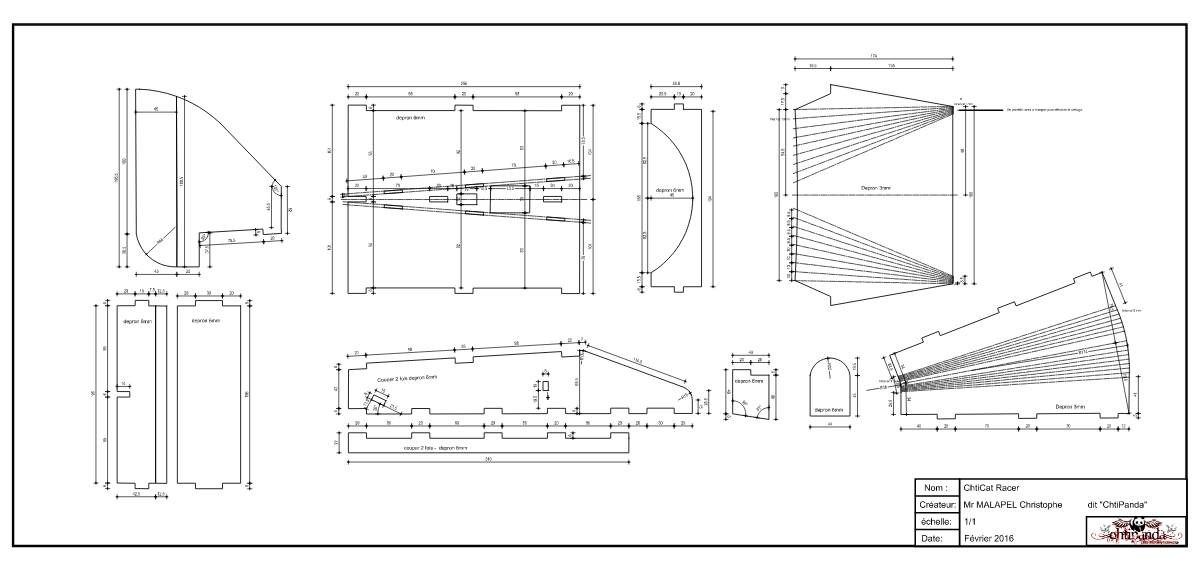
\includegraphics[width=0.5\textwidth]{../Illus/Source_Chticat}
				  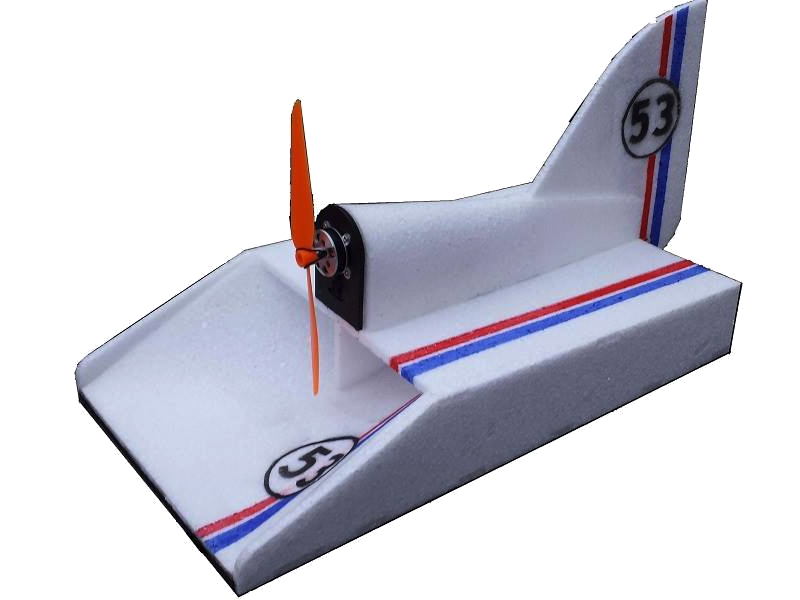
\includegraphics[width=0.3\textwidth]{../Illus/Chticat}
			\end{center}
			\caption{Mise en plan (\textit{Source :} \cite{PLCHTI}) et photo (\textit{Source :} \cite{chticat}) du \textbf{Chticat}}
			\label{MEPChticat}
		\end{figure}
		Ces plans ne peuvent pas être utilisés tel quel, en effet, nous n'utilisons pas le même matériau pour la structure, dans notre cas du carton plume et non pas du polystyrène expansé. De plus les dimensions ne sont pas strictement identiques. Et l'encombrement de notre système de contrôle est plus important que le système prévu de base pour le Chticat. En effet, le système prévu est sensé se loger sous le "dôme" central qui est bien trop petit pour nos composants. Nous avons donc décidé de redessiner les plans afin d'adapter au mieux le modèle.
		\section{Nos modifications}
		Toutes les modifications que nous avons apporté au modèle ont été réalisé sur le logiciel de \textit{Conception Assistée par Ordinateur} \href{https://freecadweb.org/}{FreeCAD} en re-modélisant les pièces du modèle originel et en modélisant de nouvelles.
			\subsection{Dimension}
				\paragraph{Matériau}Dans un premier temps, il faut prendre en compte le changement d'épaisseur du matériau. Le polystyrène expansé n'a pas la même épaisseur que le carton plume, il faut donc changer la largeur de toutes les encoches.
				\paragraph{Logement de l'électronique} Dans un second temps, nous devons repenser la \textit{cabine} qui contient l'électronique. nous avons décider de créer une \textit{cabane} sur le dessus de notre aéroglisseur. Nous pouvons voir sur la vue 3D ci dessous que nos empreintes de cartes occupent un espace optimisé dans l'intérieur de notre aéroglisseur.
				\begin{figure}[h]
					\begin{center}
						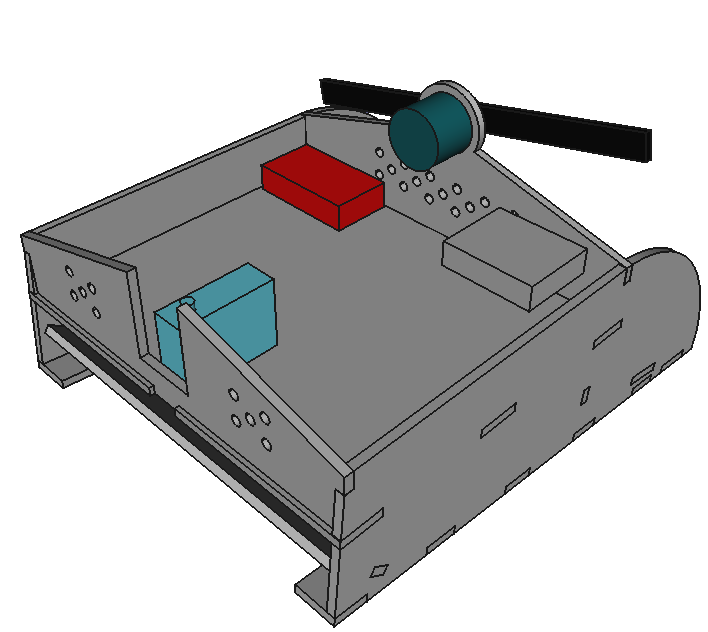
\includegraphics[width=0.85\textwidth]{../Illus/vueInterne.png}
%A METTRE A JOUR
					\end{center}
					\caption{Intérieur de notre aéroglisseur avec les empreintes des cartes}
					On peut voir respectivement en rouge, bleu et turquoise, la batterie, le servomoteur et le Brushless
					\label{MEPnous}
				\end{figure}
			\subsection{Ventilation}
			Afin de garantir un meilleur refroidissement de l'électronique, nous avons aménagé une série de trous d'aération permettant la circulation de l'air au travers de l'électronique. Ces évents sont situés juste derrière l'hélice.
			\subsection{Sécurité} Une cordelette pend derrière l'aéroglisseur. En tirant sur cette cordelette, on débranche un jumper, qui désactive le moteur de propulsion. Cette fonctionnalité est définie dans le paragraphe \ref{AU}, dans la partie contrôle. De plus, un grillage est prévu autour de l'hélice pour en assurer la protection.
			\begin{figure}[h]
					\begin{center}
						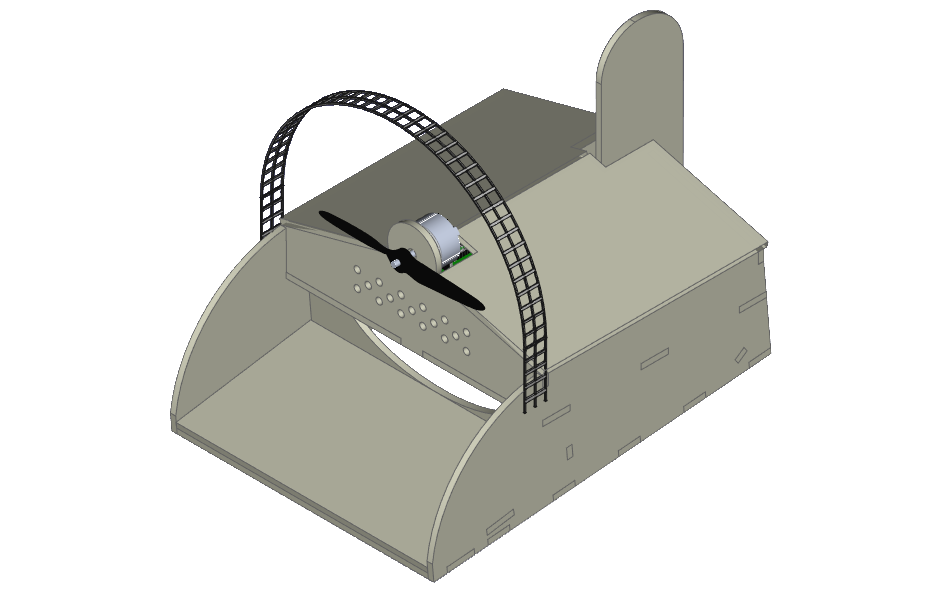
\includegraphics[width=0.9\textwidth]{../Illus/AeroProt.png}
					\end{center}
					\caption{Vue avec le grillage}
				\end{figure}
			\subsection{Modèle final}
			\begin{figure}[h]
					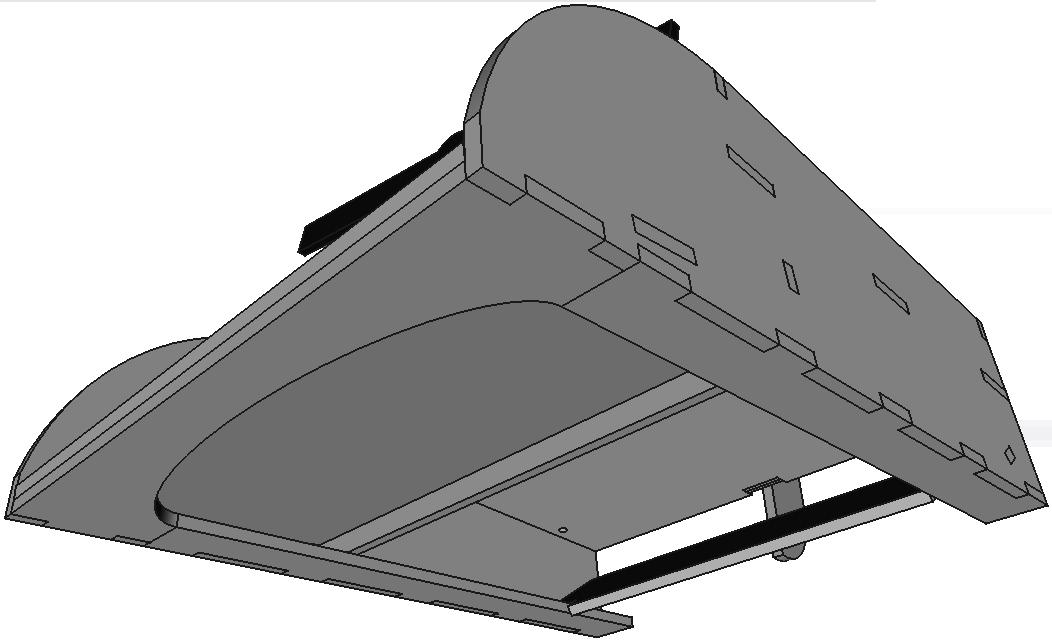
\includegraphics[width=0.24\textwidth]{../Illus/vuedessous}
					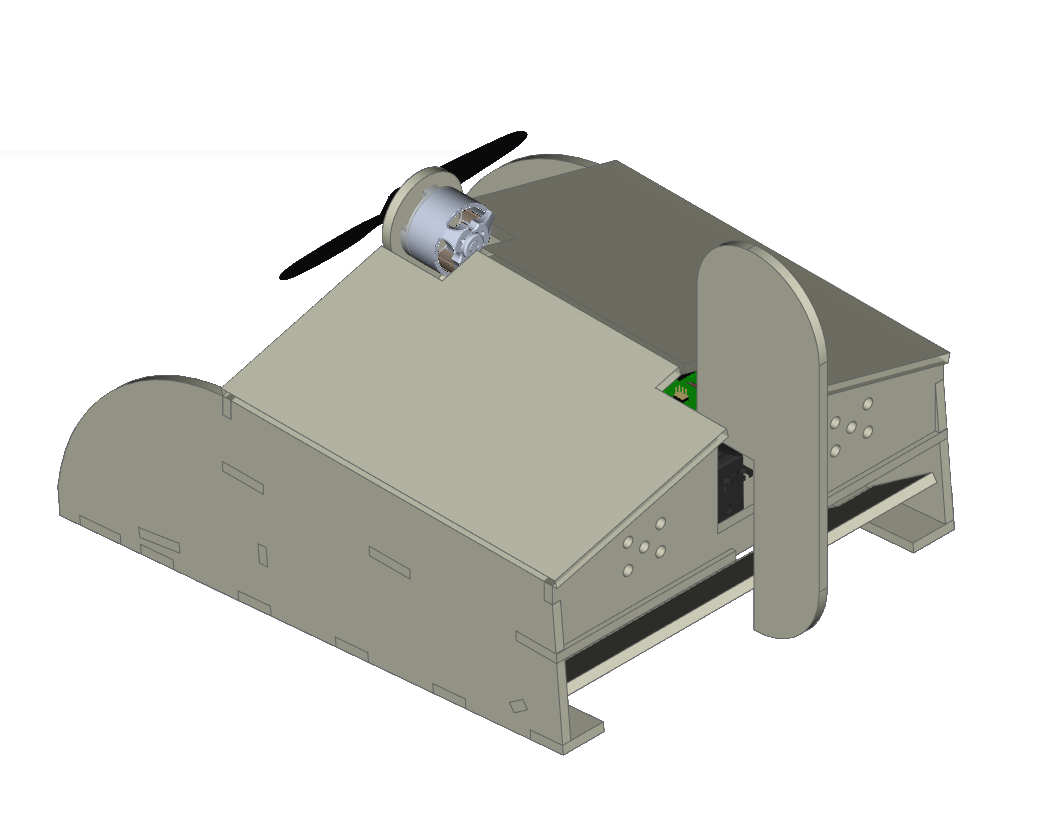
\includegraphics[width=0.24\textwidth]{../Illus/vuedessusa}
					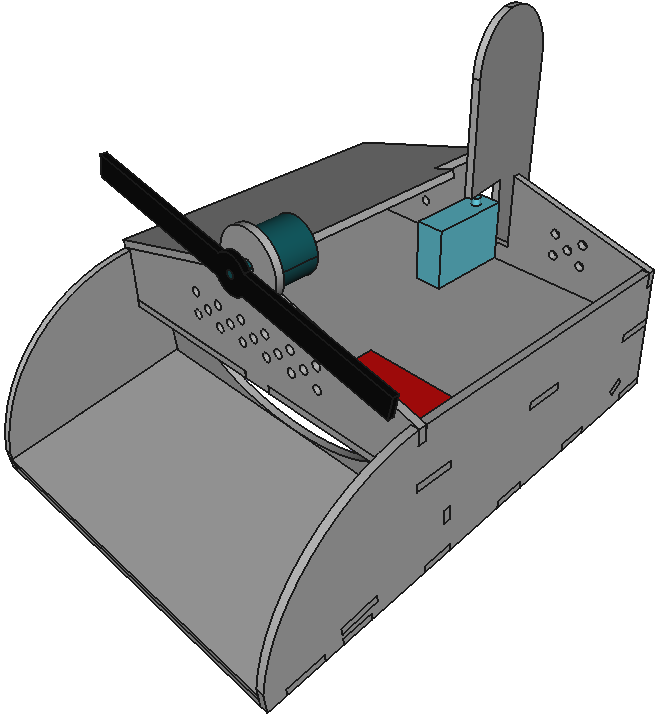
\includegraphics[width=0.24\textwidth]{../Illus/vuedessus}
					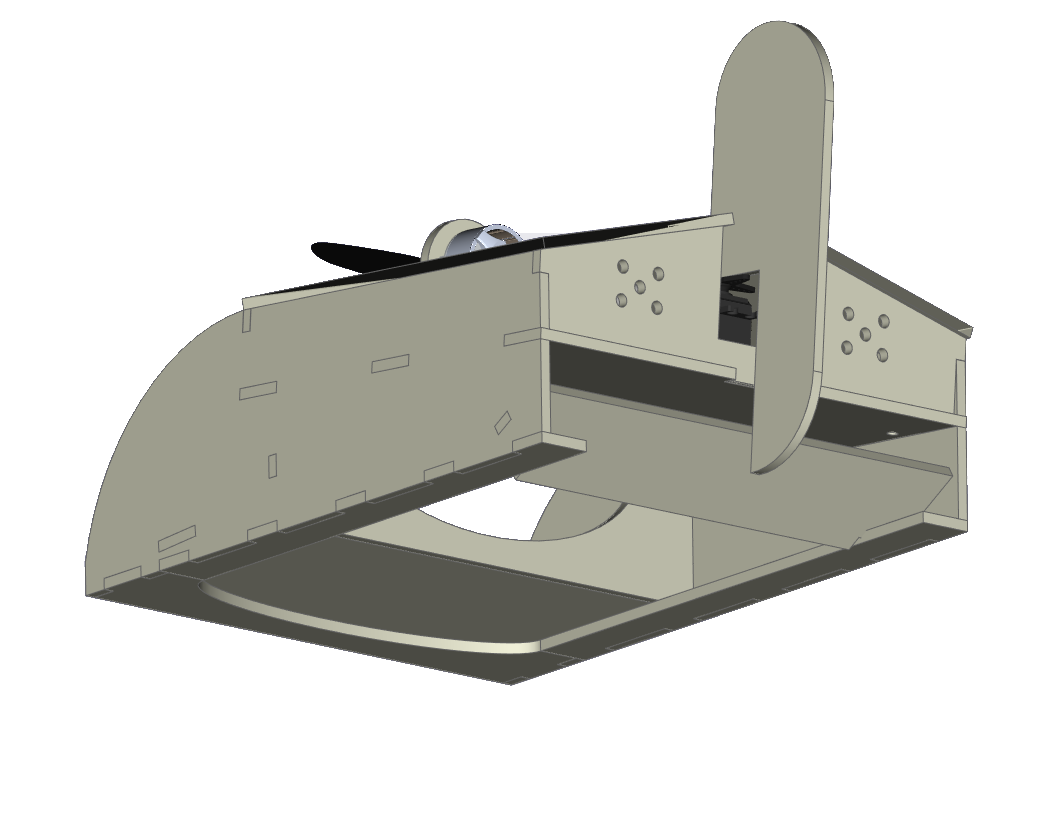
\includegraphics[width=0.24\textwidth]{../Illus/vuedessousa}
					\caption{Vues 3D de notre aéroglisseur}
					\label{vues}
				\end{figure}
				\begin{figure}
					\begin{center}
						 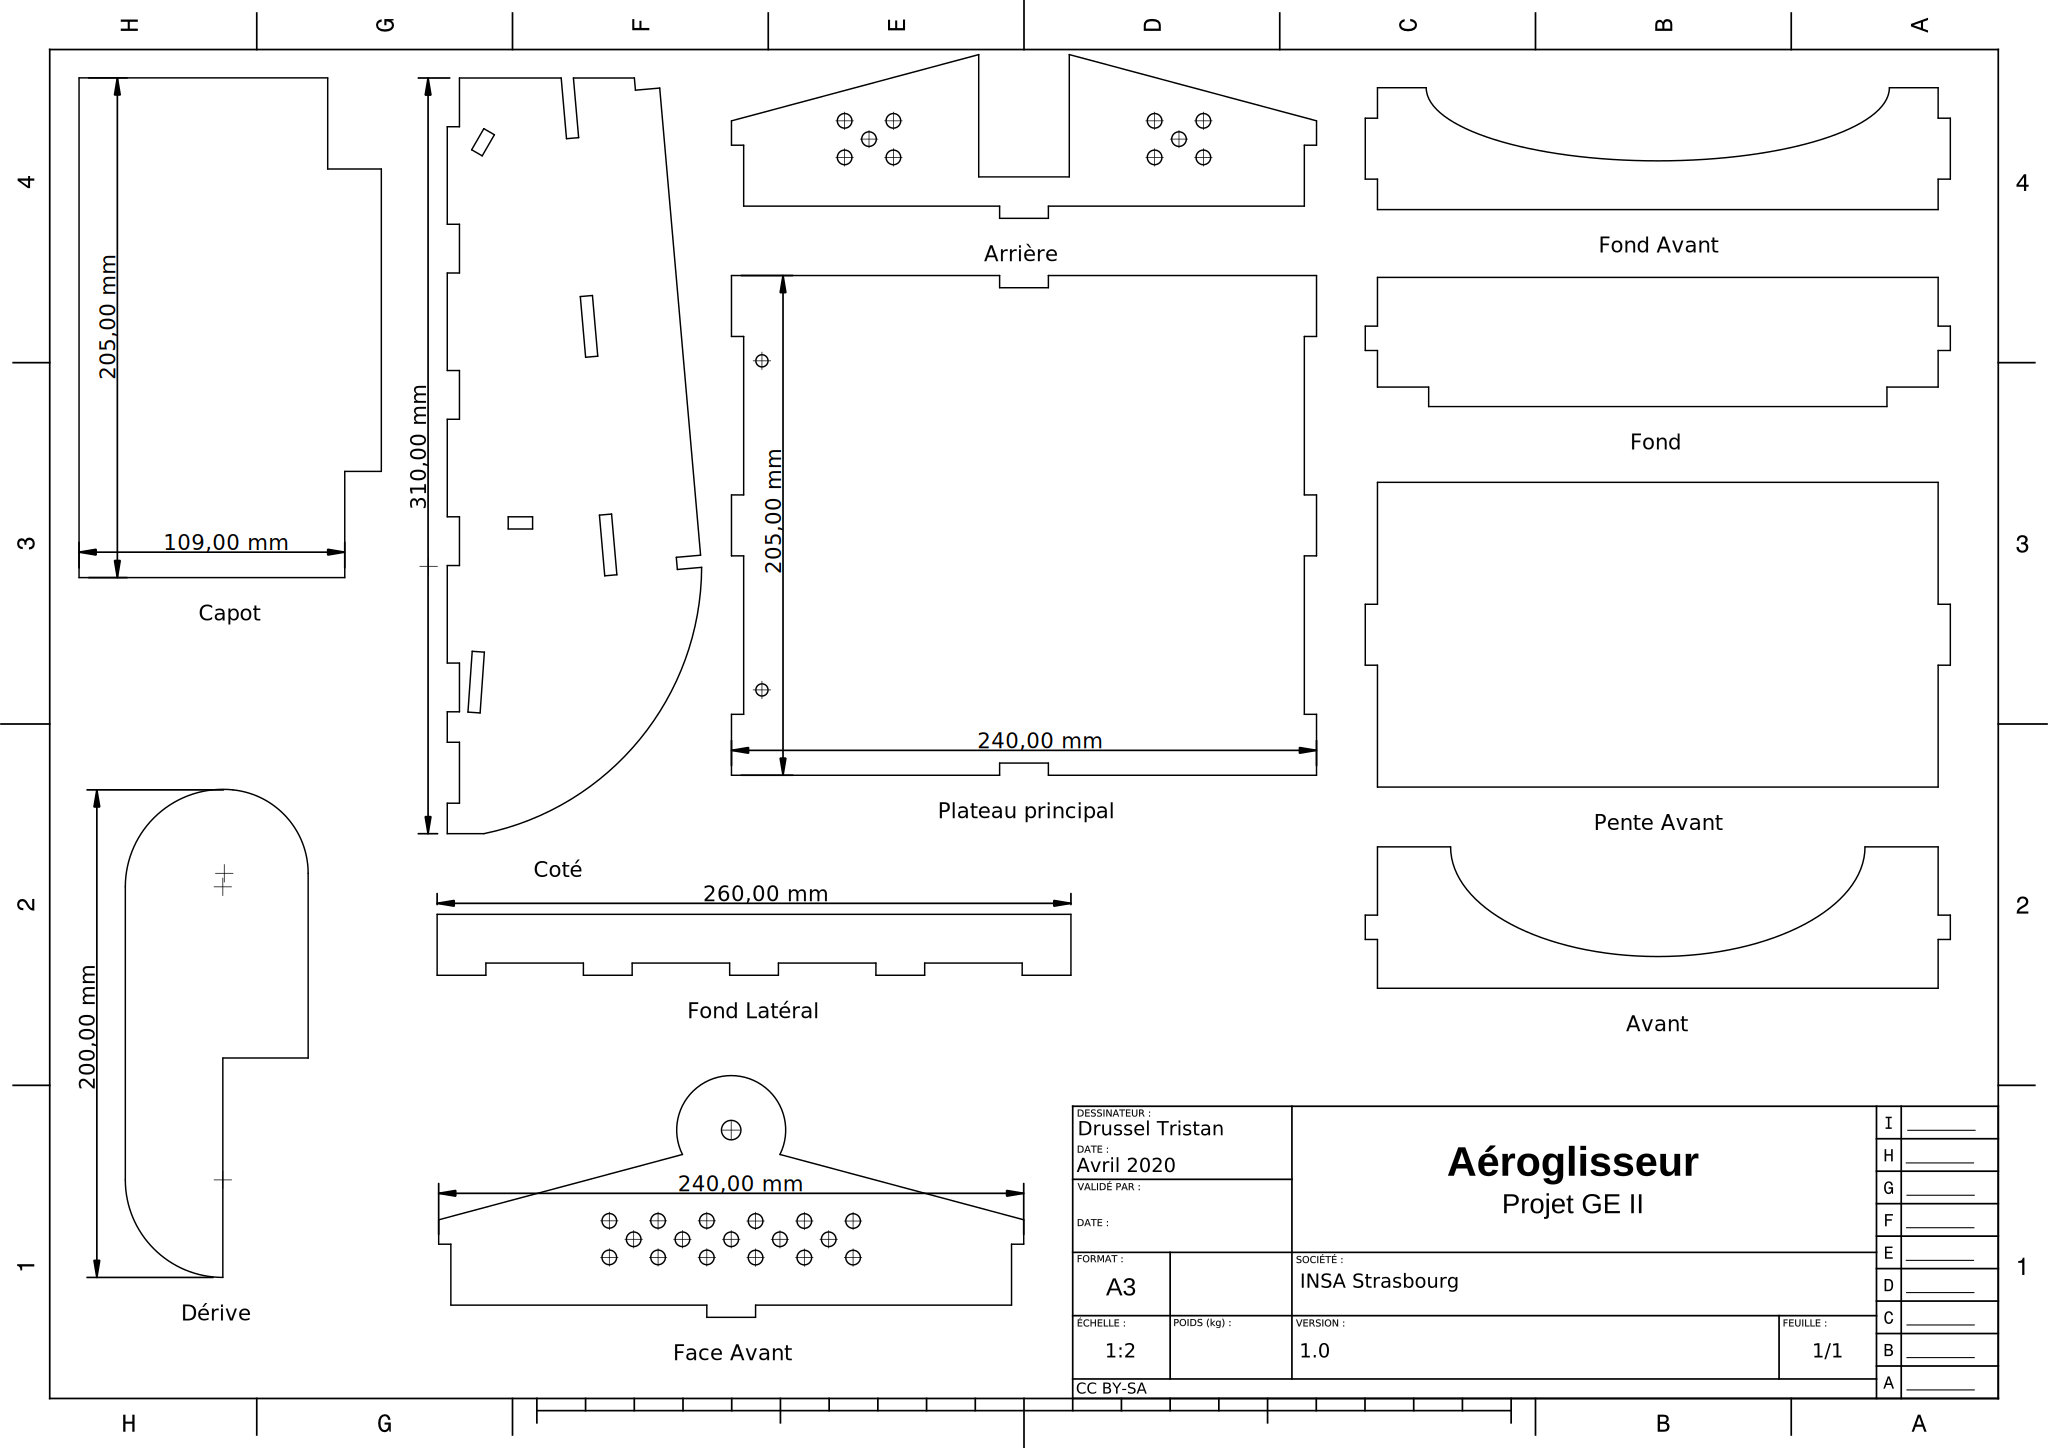
\includegraphics[width=0.5\textwidth]{../Illus/MiseEnPlanModif}
						 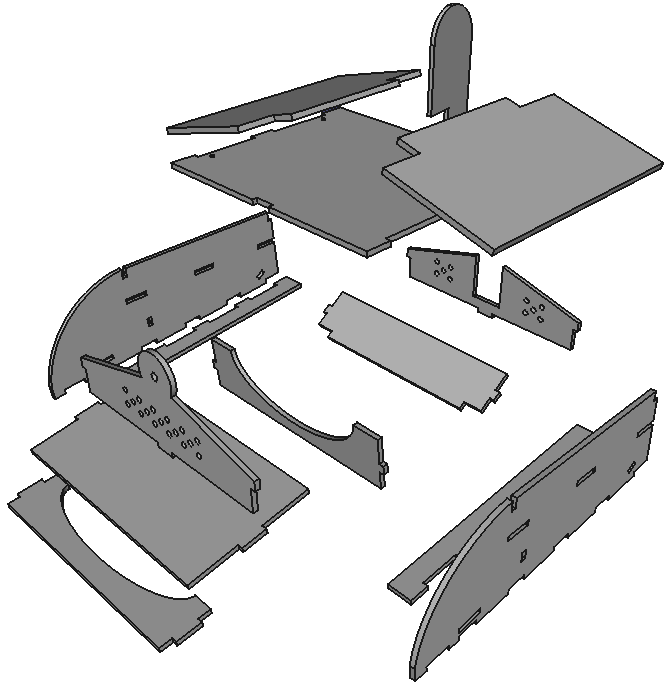
\includegraphics[width=0.3\textwidth]{../Illus/eclate}
					\end{center}
					\caption{Mise en plan et vue éclatée de notre version}
					\label{MEP}
				\end{figure}
				Notre version modifiée du Chticat répond donc au cahier des charges. Il est réalisable en carton plume de 5mm. Il permet de supporter toute l'électronique. L'hélice est protégée. Les dimensions extérieurs de la structure sont conformes au cahier des charges.
				Notre objectif était de découper le pièce en carton plume à la découpeuse Laser. Le laser étant plus rapide, précis et soigneux que nous, nous aurions pu avoir des pièces nettes et semblables à notre modélisation 3D.
				\paragraph{Assemblage} Une fois les pièces découpées, nous aurions procédé à l'assemblage des différentes pièces avec de la colle chaude. L'assemblage s'effectue autour du plateau principal, en ajoutant les fonds, les cotés l'avant et l'arrière. Dans un premier temps les capots ne seraient pas fixés afin de faciliter l'accès aux cartes. Sur le plateau principal, des petits trous sont aménagés afin de pouvoir faire passer les câbles d'alimentation des LEDs disposées à l'avant et à l'arrière. Il faut ensuite assurer la sécurité de l'hélice en fixant du grillage.